\chapter{Umsetzung}\label{ch:experiments}

Nach dem Abschluss der Spezifizerung der Benutzeranforderungen wird nun in den dritten Schritt des Human-centered design process übergegangen.
Hier gilt es, dass UX Design zu erstellen, wobei der Style Guide bereits im Ende des letzten Artikels fertiggestellt wurde.
In den folgenden Abschnitten werden noch die benötigten Interaktionsmöglichkeiten definiert und ein, auf diesen Erkenntnissen aufbauender Prototyp erstellt.

Der Großteil der Anpassungen wird in Form eines Prototypen umgesetzte, um weiterer Evaluierungen leichter durchführen zu können und um eventuelle Anpassungen innerhalb kommender Iterationen leichter umsetzen zu können.
Konkret werden die große Anpassungen der Multiselektion und die kleine Änderungen für die Template Properties innerhalb des Prototypen umgesetzte und untersucht, der Filter für die Widget Feature Properties hingegen wird direkt implementiert.
Dies hat den Hintergrund, dass es bei der Multiselektion absehbar ist das hier noch einige Anpassungen nötig sein werden, bis das Design und die Funktionalität an die Bedürfnisse des Nutzer angepasst sein wird, da hier noch keinerlei Grundlagen in EB Guide vorhanden sind auf denen aufgebaut werden kann.
Bei den Template Properties hat die Umsetzung innerhalb des Prototypen den Hintergrund, das hier nicht sicher gesagt werden kann ob die Verlagerung der Funktion \glqq publish to template interface\grqq{} von den Nutzern tatsächlich angenommen oder überhaupt an der neuen Stelle intuitiv erwartet wird.
Es ist hier auch sehr wahrscheinlich das an der Darstellung, Position und der Kombination mit der alten Position noch einige Anpassungen stattfinden müssen.
Daher macht es Sinn, sich bei diesen beiden Anpassungen strikt an den Human-centered design process zu halten und innerhlab dessen Iterationen solange das UX design zu verbessern bis es sicher den Nutzeranforderungen entspricht.
Ansonsten würde hoher Entwicklungsaufwand in Anpassungen fließen die noch häufig angepasst oder komplett verworfen werden müssen.
Die Anpassung des Prototypen kann in diesen Fällen schneller, minimalistischer und mit kleinerem Aufwand erfolgen.

Im Gegensatz dazu ergibt es Sinn die Filterfunktion direkt in EB Guide zu implementieren.
Aus den bereits durchgeführten Analysen geht hervor, dass dieser Filter einen großen Mehrwert für die Nutzer bieten würde.
Im Gegensatz zu den beiden anderen Änderungen ist auch am Design dieser Änderungen kein großer Spielraum mehr für Anpassungen, da sich das Design hier an den bereits bestehenden Filter und Suchfunktionen innerhalb von EB Guide orientiert.
Die einzige eventuelle Änderungen die hier noch auftreten könnte wäre eine Änderung der Position.
Ob diese Anpassungen jedoch innerhalb eines Prototypen oder im XAML Code stattfindet macht, betrachtet man den zeitlichen Aufwand, keinen Unterschied.
Daher ist es für diese Änderung in diesem Fall effizienter die Änderungen direkt zu implementieren und das Verhalten nicht zuerst innerhalb eines Prototypen zu simulieren.

\section {Prototyp Multiselektion und Template Properties}
In den folgenden Abschnitten wird alles Relevante in Bezug, auf die im Prototpy umgesetzten Änderungen erläutert.
Zuerst gibt es keine kurze Begründung für die Wahl des Prototyping Tools, bevor dieses noch kurz in seinen Grundfunktionen erläutert wird.
Danach werden die nötigen Interaktionsmöglichkeiten erläutert, die dem Nutzer für einen erfolgreichen Umgang mit dem Prototypen simuliert werden müssen, bevor letztlich die Vorgehensweise beschrieben wird um diese Anforderungen umzusetzen.

\subsection {Axure RP}
Axure RP ist eine Software die es ermöglicht Wireframes, Prototypen, Dokumentationen und Spezifikationen für Web-, Mobil- oder Desktopanwendungen zu erstellen.
Dies wird durch Drag und Drop Aktionen, Skalierung und Formatierung von Widgets ermöglicht, mit deren Hilfe man das gewünschte Endprodukt erstellen kann.
Für diese Arbeit ist vor allem die Möglichkeit einen Prototypen zu erstellen wichtig.
Ausschlaggebend für die Wahl dieser Software war, dass AXURE RP 9 die Möglichkeit bietet dynamische Inhalte zu erstellen und logische Bedingungen in den Prototypen einzubinden.
Da es sich bei EB Guide Studio um ein Modellierungstool handelt ist ein rein statischer Prototyp nicht ausreichend.
Ebenfalls reicht es nicht aus feste Hotspots zu haben bei deren Klick etwas passiert, sondern es ist notwendig die in EB Guide herrschenden Einschränkungen für den Nutzer simulieren zu können.

Ein weiterer Grund sich für diese Software zu entscheiden war es, das die UX Designer bei Elektrobit ebenfalls mit AXURE RP arbeitet.
So war es zum einen gewährleistet das bei den Usabilitytest keine Schwierigkeiten mit der verwendeten Software auftreten würde, zum anderen war dadurch gleichzeitig ein Ansprechpartner bei auftretenden Problemen vorhanden.

In \cref{fig:Axure_Full} ist das Standardprojekt von AXURE RP zu sehen, welches die Grundlage eines jeden neuen Projektes bildet.

\begin{center}
  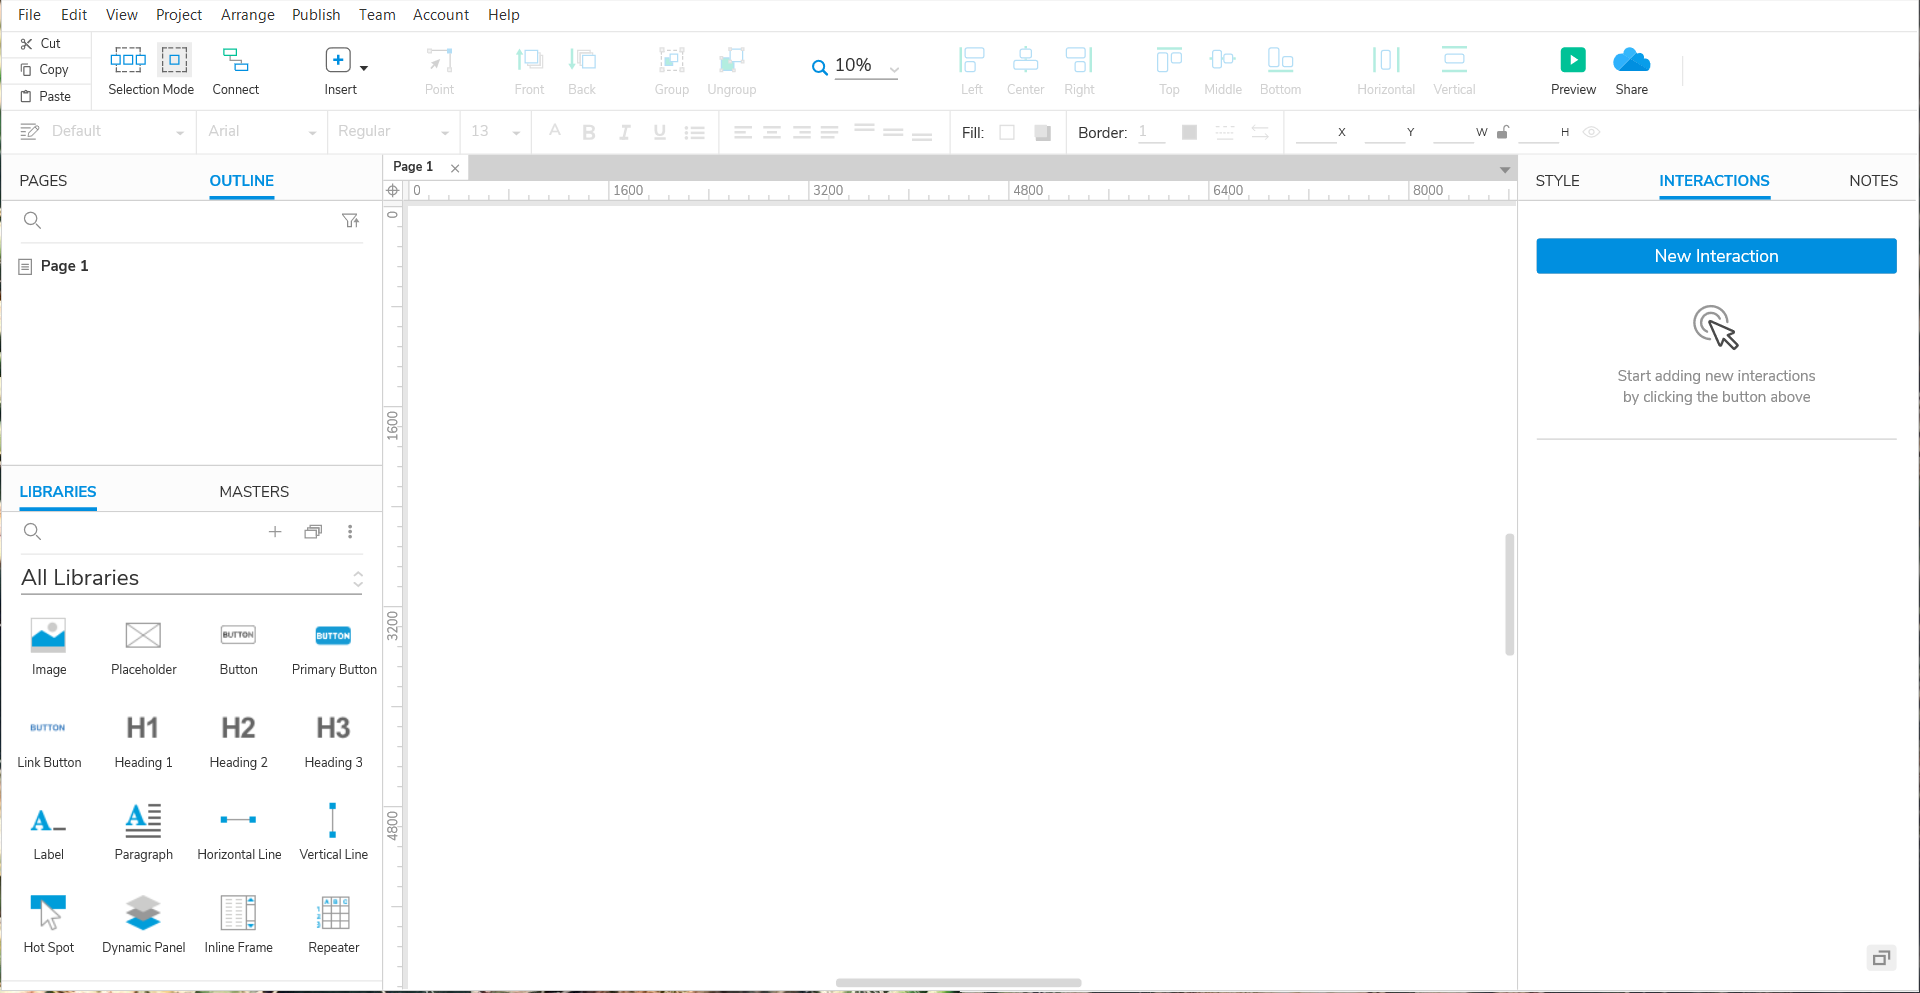
\includegraphics[scale=0.4]{figures/Axure_Full.png}
  \captionof{figure}{Axure RP 9}
  \label{fig:Axure_Full}
\end{center}

In den mittig platzierten Workspace können Elemente aus den Libraries links oder eigene, externe Elemente eingefügt werden.
Zieht man nun beispielsweise eine Droplist und drei Kreiselemente aus den Libraries links in den Workspace passt sich die Outline wie in \cref{fig:Axure_Outline} zu sehen entsprechend an.
Mithilfe dieser Outline kann man innerhalb des Projektes navigieren, was vor allem praktisch ist wenn sich mehrere Elemente, wie auch in diesem Beispiel zu sehen, überlagern.
Elemente lassen sich auch zu Dynamic Panels gruppieren, was vor allem dann nötig ist wenn man ein Drag und Drop Verhalten simulieren möchte, da dies die einzigen Widgets sind die dieses Verhalten unterstützen.

\begin{center}
  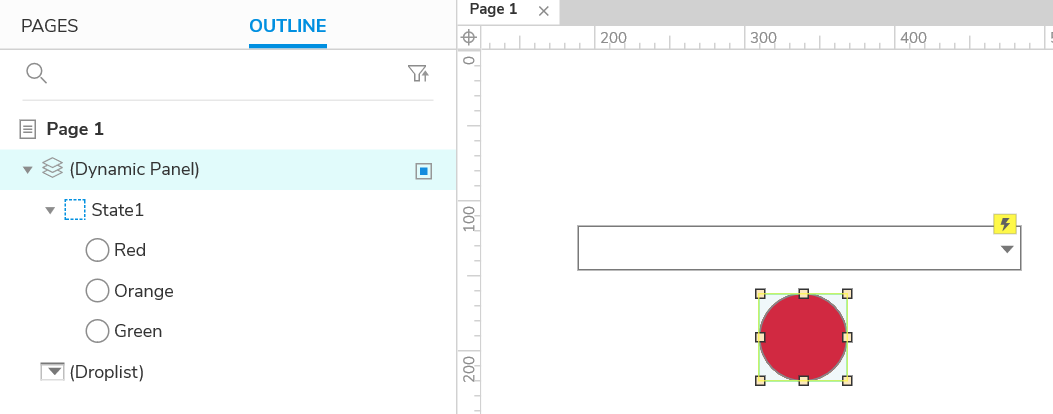
\includegraphics[scale=0.4]{figures/AXURE_Outline.PNG}
  \captionof{figure}{Axure RP 9 Outline}
  \label{fig:Axure_Outline}
\end{center}

Um den drei eingefügten Kreisen unterschiedliche Farben zuzuweisen ist es nötig deren Properties zu bearbeiten.
Die ist in AXURE RP über das Stlye Panel möglich, welches in \cref{fig:Axure_Style} zu sehen ist.
Hier ist es beispielsweise ebenfalls möglich Skalierungen vorzunehmen, oder Umrandungen und Schatten hinzuzufügen.

\begin{center}
  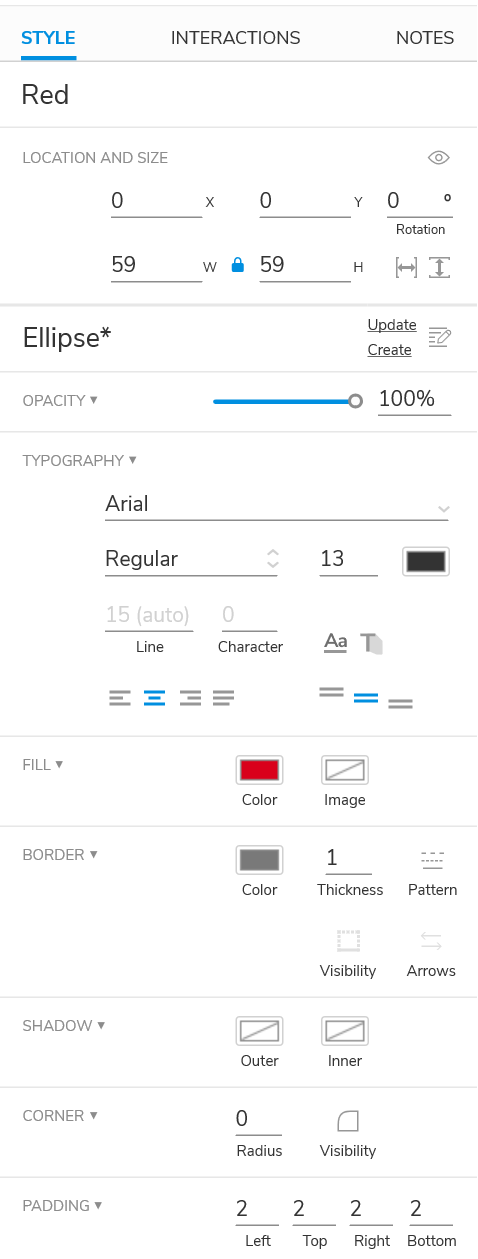
\includegraphics[scale=0.4]{figures/AXURE_Style.PNG}
  \captionof{figure}{Axure RP 9 Style Properties}
  \label{fig:Axure_Style}
\end{center}

Wenn man nun erreichen möchte, das die Farbe des sichtbaren Kreises ich an der Auswahl innerhalb der Droplist orientiert muss Logik zu dem Prototypen hinzugefügt werden.
Zuerst ist es, wie in Teil a von \cref{fig:Droplist} zu sehen, nötig Optionen innerhalb der Droplist hinzuzufügen.
Innerhalb des Interactionpanels besteht dann die Möglichkeit, über IF Conditions abzufragen, welche Option aktuell ausgewählt ist und die Visibility der Kreise entsprechend zu regulieren.

\begin{figure}%
\centering
\subfloat[][]{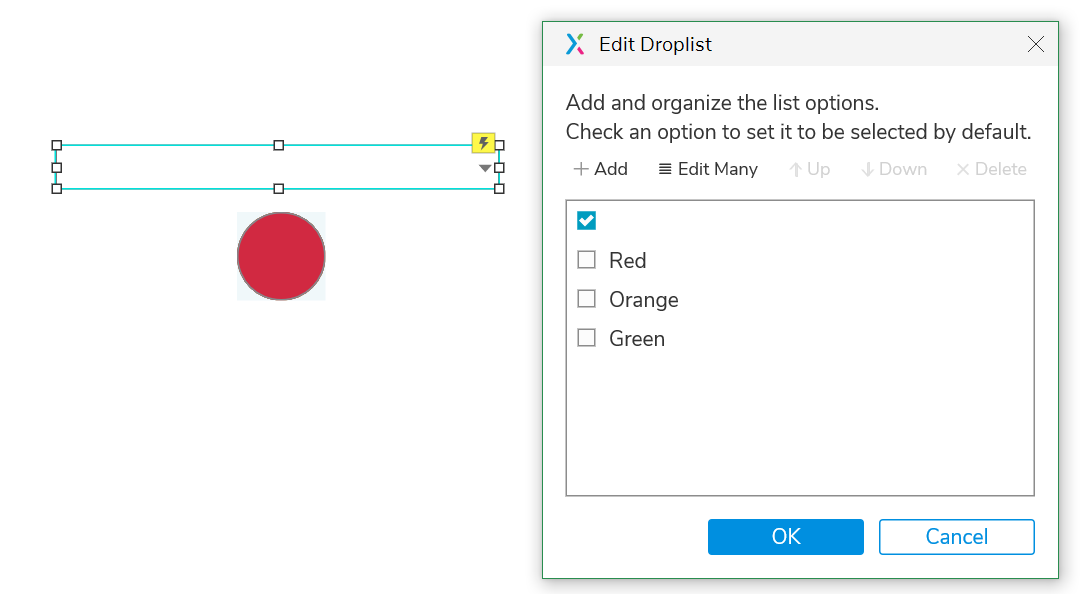
\includegraphics[width=0.5\linewidth]{figures/AXURE_Droplist.PNG}}%
\qquad
\subfloat[][]{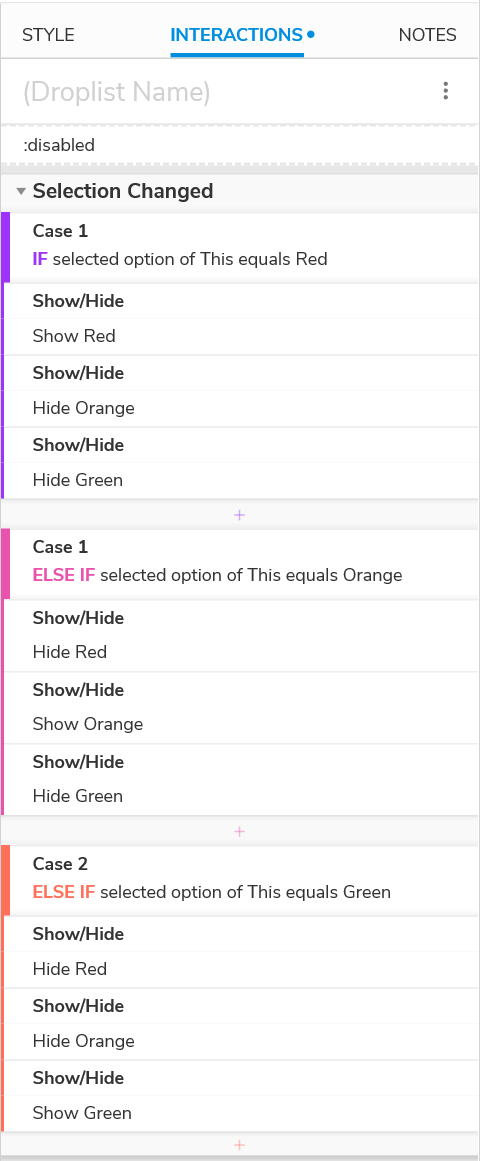
\includegraphics[width=0.3\linewidth]{figures/AXURE_Droplist_Conditions.PNG}}%

\caption{Axure RP Droplist und Conditions}%
\label{fig:Droplist}
\end{figure}

Hat man die Modellierung abgeschlossen, oder möchte etwas überprüfen, bietet AXURE RP die Möglichkeit einer lokalen Preview.
Diese verhält sich exakt so, wie sich der abgeschlossene Prototyp ebenfalls verhalten wird und eignet sich deshalb gut für selbständige Validierung der bisherigen Umsetzung.
Testet man das soeben modellierte Beispiel in der Preview sieht man in \cref{fig:Droplist} , dass sich die Farbe des Kreises, wie gewünscht, immer an die Auswahl der Droplist anpasst.
\begin{figure}%
\centering
\subfloat[][]{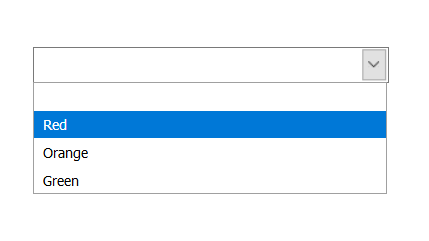
\includegraphics[width=0.3\linewidth]{figures/AXURE_red.PNG}}%
\qquad
\subfloat[][]{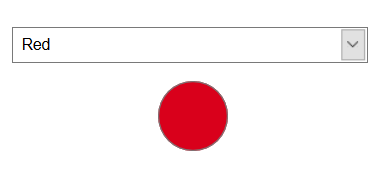
\includegraphics[width=0.3\linewidth]{figures/AXURE_red02.PNG}}%
\qquad
\subfloat[][]{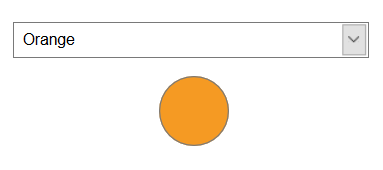
\includegraphics[width=0.3\linewidth]{figures/AXURE_orange.PNG}}%
\qquad
\subfloat[][]{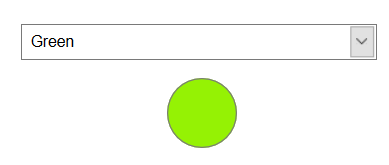
\includegraphics[width=0.3\linewidth]{figures/AXURE_green.PNG}}%

\caption{Axure RP Preview}%
\label{fig:Preview}
\end{figure}

Ist die Modellierungsarbeit beendet bietet AXURE RP die Möglichkeit, dass Projekt in die AXURE CLOUD zu laden.
Hier können andere Mitarbeiter über einen generierten Link auf das funktionale Endprodukt zugreifen, ohne das eigentliche Projekt sehen oder bearbeiten zu können.
Dadurch ist es nun einerseits möglich andere UX Designer Funktionalitäten des Prototypen testen zu lassen, wobei sie auch an den entsprechenden Stellen Kommentare und TODO's hinterlassen können.
Außerdem besteht durch den Link die Möglichkeit den Prototypen für die Testpersonen im Rahmen des Usability Tests zugänglich zu machen.

\subsection{Interaktionsmöglichkeiten}

Im dritten Schritt des Human-centered design process ist es die Aufgabe des Interaction Designers die Interaktionsmöglichkeiten, die der Prototyp bieten muss, zu spezifizieren.
Dies ist deshalb notwendig, da es gerade bei Prototypen die ein komplexes System simulieren sollen, nicht möglich oder nötig ist alle Funktionen des Systems zu simulieren.
Daher wird vor der Erstellung des Prototyps festgelegt welche Interaktionen von den Nutzern durchführbar sein müssen um die geplanten Verbesserungen validieren zu können.

Für die Überprüfung der Usability der Ergänzungen ist es jedoch nicht ausreichend nur die neuen oder ergänzten Funktionen zu simulieren.
Um diese Ergänzungen überhaupt anwenden zu können muss der Nutzer einen gewissen Punkt innerhalb des Modellierungsprozesses erreicht haben.
Um an diesen Punkt zu gelangen ist es unbedingt notwendig, dass dem Nutzer gewissen Grundfunktionen von EB Guide zur Verfügung stehen.
Das bedeutet für den konkreten Fall dieser Bachelorarbeit, dass es für den Nutzer möglich sein muss wie gewohnt Elemente per Drag and Drop in den View zu ziehen, und diese dort auch frei bewegen zu können.
Ebenfalls müssen die Properties aller Widgets frei anpassbar sein und die Elemente müssen wie gewohnt auf die Eingaben des Nutzers reagieren.
Das sich die Funktionen \glqq publish to template interface\grqq{} innerhalb der Templates befindet, muss auch die Möglichkeit bestehen Templates anzulegen.

Darauf aufbauend müssen noch die neuen oder veränderten Funktionen in den Prototypen integriert werden.
Dazu zählt konkret, dass die Funktion \glqq publish to template interface\grqq{} verlagert wird und die alte Möglichkeit dafür vorerst nicht simuliert werden muss.
Zusätzlich muss es nun möglich sein mehrere Elemente gleichzeitig auszuwählen und hierfür ein Propertiepanel einzublenden.
Die Anpassung der Properties müssen sich in diesem Fall auch auf alle angewählten Elemente auswirken, und diese müssen auch gemeinsam im View bewegt werden können.
Zusätzlich müssen noch die neuen Alignment Actions, sowie die Funktion Insert in Template angezeigt werden und ausführbar sein.

Da sehr viele unterschiedliche Widget- und Templatetypen in EB Guide existieren, ist es an dieser Stelle des Prozesses auch sinnvoll sich bereits grobe Gedanken über den abschließenden Usability Test zu machen, und die Funktionen des Prototypen entsprechend einzuschränken.
Da die Modellierer bei Elektrobit hauptsächlich HMIs für den Fahrzeuginnenraum mit EB GUIDE umsetzen, erscheint es sinnvoll für den Usability Test einen minimalistischen Startscreen eines solchen Interfaces modellieren zu lassen.
Da diese, wenn man die Interaktionslogik außen vor lässt, nur aus Images und Labels bestehen ist es ausreichend diese beiden Widgets funktionsfähig zu machen.
Zusätzlich dazu ist es noch notwendig die Menge an verfügbaren Templates einzuschränken.
Für den soeben erläuterten Use Case ist es hier ebenfalls ausreichend nur Image Templates erstellen zu können.
Genauere Erläuterungen zu den Aufgaben innerhalb des Usability Test folgen entsprechend in Kapitel 5 dieser Arbeit.


\subsection{Vorgehensweise}
Im folgenden werden die gurndlegenden Vorgehensweisen erläutert die angewandt wurden um den letztendlichen Prototypen zu erstellen.
Es ist im Rahmen dieser Arbeit nicht möglich alle Anpassungen zu erläutern die getätigt werden mussten, es werden jedoch die maßgeblichen Konzepte und Funktionen vor allem in Bezug auf die wichtigsten Anpassungen aufgeführt.

Vor allem bei Expertennutzern ist es wichtig, das der Prototyp sich nicht nur verhält wie die  gewohnte Software, sondern sich auch optisch an ihr orientiert.
Von daher war der Ansatz zur Modellierung des Prototypen einen Screenshot von der aktuellen Version von EB GUIDE Studio zu machen und diesen als statischen Hintergrund, wie in \cref{fig:Prototyp_01} zu sehen, für das weitere Vorgehen zu benutzen.
Darauf aufbauend können nach und nach Interaktionsmöglichkeiten innerhalb des Prototypen platziert werden.

\begin{center}
  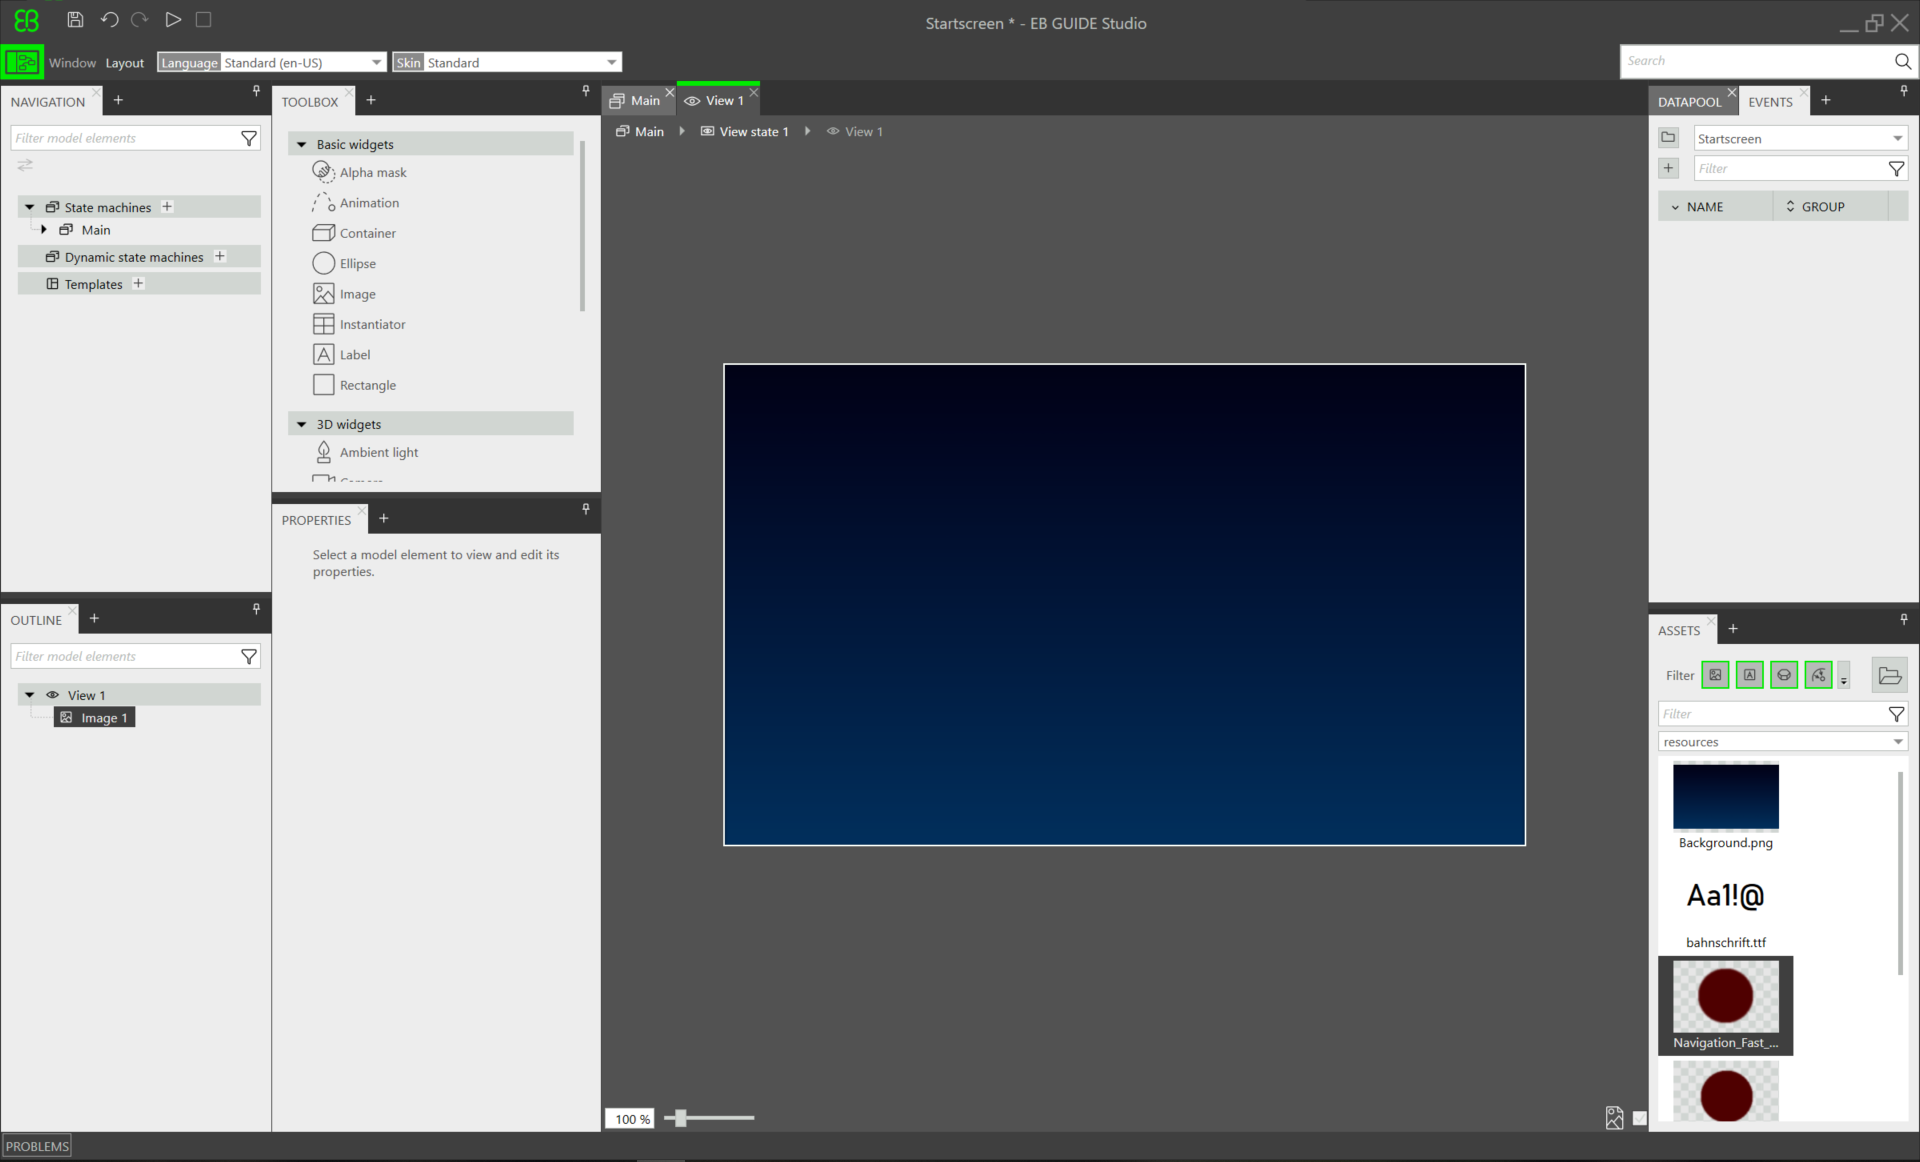
\includegraphics[scale=0.4]{figures/Prototyp_01.PNG}
  \captionof{figure}{Grundlage des Prototyps}
  \label{fig:Prototyp_01}
\end{center}

Die Assets und die Toolbox sind wichtige Interaktionsmöglichkeiten für den Nutzer, da von hier aus alle zur Verfügung stehenden Widgets oder Ressources in den View gezogen werden.
Für beide Elemente wird eine Scrollbar benötigt, da dies aufgrund der Masse der Widgets in EB GUIDE ebenfalls bereits so gelöst ist.
In AXURE ist es hierfür nötig ein Dynamic Panel zu erstellen und es mit allen benötigten Elementen zu befüllen die in der Scrollbar vorhanden sein sollen.
Für ein Dynamic Panel ist es möglich eine feste Größe anzulegen, sollten dessen Elemente in der vorgegebenen Dimension nicht alle Platz finden hat man nun die Möglichkeit Vertikales oder Horizontales Scrolling zu aktivieren.
In \cref{fig:Prototyp_02} sieht man beispielhaft die Umsetzung für das Assetspanel.
Teil a) zeigt die Implementierung mithilfe von ineinander geschachtelter Dynamic Panels, in Teil b) ist das entsprechende Ergebnis im Prototypen zu sehen.

\begin{figure}%
\centering
\subfloat[][]{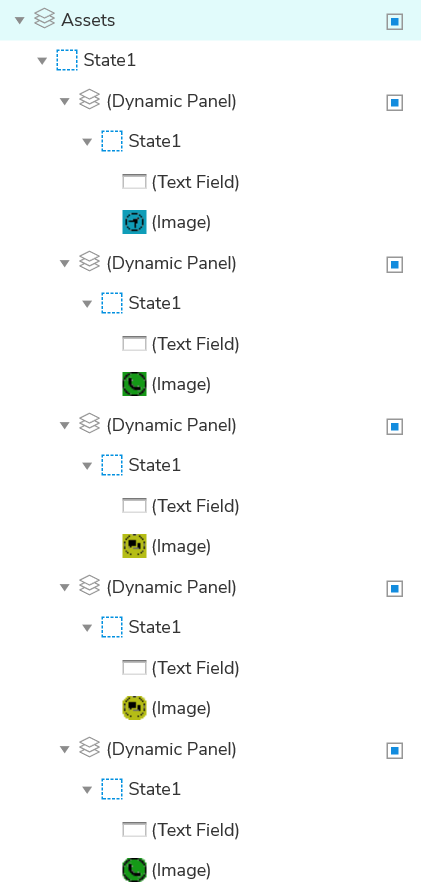
\includegraphics[width=0.4\linewidth]{figures/Prototyp_Assets.PNG}}%
\qquad
\subfloat[][]{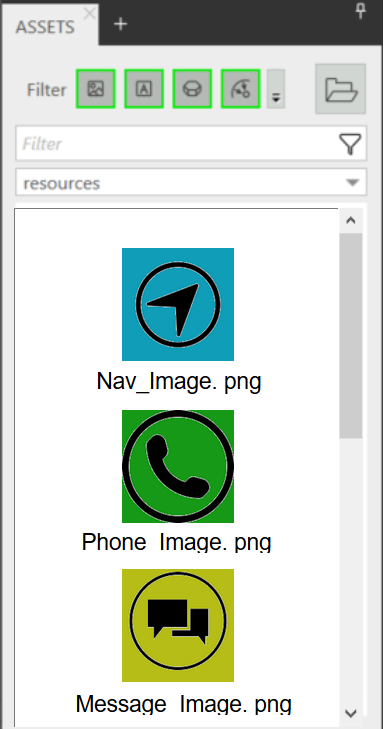
\includegraphics[width=0.4\linewidth]{figures/Prototyp_02.PNG}}%

\caption{Scrollbar für Assets}%
\label{fig:Prototyp_02}
\end{figure}

Der Grund dafür das jedes einzelne Bild in den Assets ebenfalls ein Dynamic Panel ist, ist der Tatsache geschuldet das dies die einzigen Widgets sind die Drag und Drop unterstützen.
Sie bieten die einzigartigen Interactions \glqq Drag Started\grqq{},\glqq Dragged\grqq{} und \glqq Drag Dropped\grqq{} über welche gesteuert werden kann wie sich die Items während des Vorgangs verhalten.
Hier erweist es sich vor allem als praktisch \glqq Drag Dropped\grqq{} mit einer If Bedingung zu versehen, damit das Element nur über dem dafür vorgesehenen View abgelegt werden kann, und nicht zum Beispiel im Bereich der Datapoolitems.

Sobald etwas in den View etwas hinzugefügt wird, muss dies für den Nutzer ebenfalls im Widgettree sichtbar werden.
In \cref{fig:Prototyp_03} is zu sehen das hier ebenfalls wieder mit einem Screenshot aus dem tatsächlich EB GUIDE gearbeitet wurde, die gelben Pfeile markieren bestehende Interaktionen in AXURE.
Man sieht, dass sich hier noch mehr Elemente im Widget Tree befinden, die vorläufig überdeckt wurden.
Fügt der Nutzer nun das entsprechende Element zum View hinzu, wird die Abdeckung entfernt und er kann das Objekt nun auch über den Widget Tree auswählen.
Diese Verhalten ist ebenfalls wieder mit logischen Bedingungen umgesetzt.

\begin{center}
  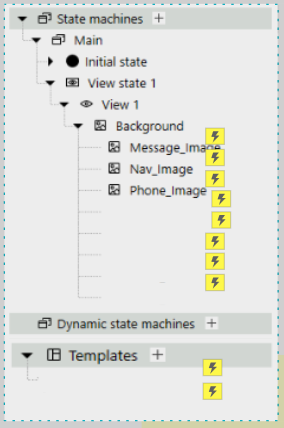
\includegraphics[scale=0.8]{figures/Prototyp_03.PNG}
  \captionof{figure}{Widget Tree}
  \label{fig:Prototyp_03}
\end{center}

Um die Interaktion mit allen eingefügten Elementen möglich zu machen, hat jedes Element sein eigenes Propertiespanel erhalten, welches in \cref{fig:Prototyp_04} zu sehen ist.
Damit dem Nutzer immer klar ist welches Element aktuell ausgewählt ist, wurde auch hier das Verhalten von EB GUIDE nachgebaut, indem jedes ausgewählte Element einen grünen Rahmen erhält.
Die Auswahl hierfür muss über das Element selbst oder den Widget Tree möglich sein, in letzterem Fall wurde das wieder über Hot Spots und logische Bedingungen umgesetzt.

Ist das Objekt aktuell ausgewählt erscheint ein entsprechendes Propertiespanel welches ebenfalls wieder einen Screenshot beinhaltet der mit Textfeldern überlagert wird.
Diese Felder sind mit globalen Variablen verknüpft, welche wiederum die Properties der Bilder im Workspace von AXURE anpassen.
Dadurch wird es ermöglicht, dass Eingaben in das Textfeld das Objekt verändern und umgekehrt, Bewegungen des Objektes die Werte in den Textfeldern aktualisieren.
Damit wird für den Nutzer das exakt gleiche Verhalten nachmodelliert welches in EB GUIDE existiert.
Das gleiche Verhalten gilt für Texte, nur haben iese statt eines Image Properties ein Text Property.

\begin{center}
  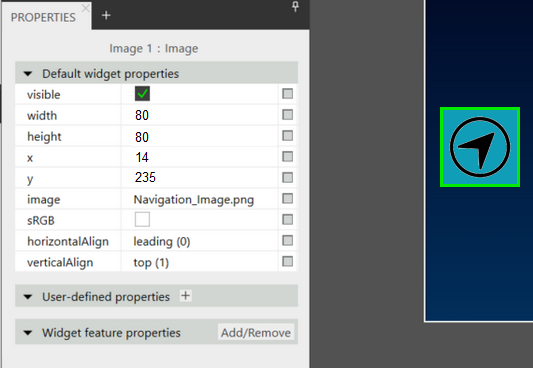
\includegraphics[scale=0.8]{figures/Prototyp_04.PNG}
  \captionof{figure}{Properties Panel}
  \label{fig:Prototyp_04}
\end{center}

Ist nur ein Objekt ausgewählt wird der Wert der globalen Variable im entsprechenden Textfeld angezeigt.
Da dieser Wert bei der Multiselektion jedoch nur angezeigt werden soll wenn er für alle ausgewählten Objekte identisch ist, und ansosnten ein Strich sichtbar sein soll, ist es hier notwendig die Properties der ausgewählten Objekte zu vergleichen.
Hierfür muss zuerst abgefragt werden welche Objekte ausgewählt sind und dann deren Properties verglichen werden.
Da AXURE bei den logischen Bedingungen nur \glqq Match Any\grqq{} oder \glqq Match All\grqq{} unterstützt ist keine Kombination von AND und OR Bedingungen möglich.
Deshalb wird an diesem Punkt nur mit AND Bedingungen in den Abfragen gearbeitet, da jedoch für alle möglichen Kombination der drei zur Verfügung stehende Bildern jede Property einzeln abgefragt und angepasst werden muss ergibt das eine Anzahl von 36 Abfragen.

\begin{center}
  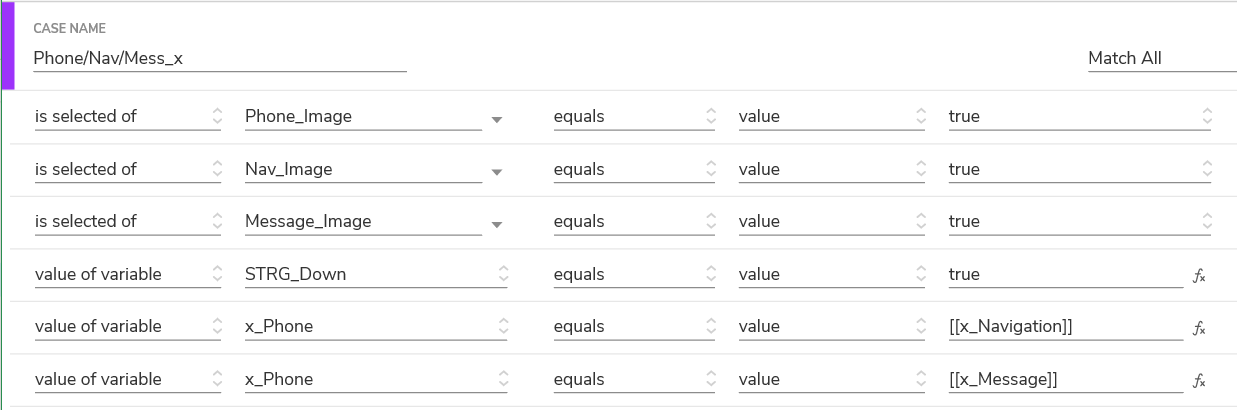
\includegraphics[scale=0.6]{figures/Prototyp_05.PNG}
  \captionof{figure}{Beispielbedingung Multiselektion}
  \label{fig:Prototyp_05}
\end{center}

Der gleiche Aufwand wird ebenfalls noch für die verfügbaren Texte betrieben.
Aufgrund der Performance des Prototyps und der Fehleranfälligkeit wurde auf diese Anpassung bei der gleichzeitigen Auswahl von Texten und Bildern verzichtet.
Es ist hier möglich die Properties anzupassen, es wird jedoch nicht verglichen ob deren Variablen den gleichen Wert aufweisen, sondern es wird immer ein Strich angezeigt.
In \cref{fig:Prototyp_05} ist beispielhaft die logische Bedingung für den Fall zu sehen das alle drei Bilder gleichzeitig ausgewählt sind und deren x-Koordinate jeweils identisch ist.

Zeitgleich mit den Properties werden bei bei der Mehrfachselektion die Alignment Actions angezeigt.
Hier wird im Prototypen die Umsetzung in Bezug auf den Testcase eingeschränkt.
Da ein Startscreen modelliert werden soll reicht die Möglichkeit die Bilder Horizontal aneinander auszurichten, die Vertikale Ausrichtung ist von Texten an Bildern möglich.
In \cref{fig:Prototyp_06} ist die Umsetzung im Prototyp zu sehen, wobei Teil a) bei zwei ausgewählten Bildern und Teil b) bei der gleichzeitigen Auswahl von Bild und Label sichtbar ist.
Die Alignment Actions liegen bei der Auswahl von zwei Objekten des gleichen Typs absichtlich unten, und bei der Auswahl von zwei unterschiedlichen oben.
Bei letzterem Fall kann eher davon ausgegangen werden das keine Properties gemeinsam angepasst werden müssen, sondern die zwei unterschiedlichen Objekte eher aneinander ausgerichtet werden sollen.
Die tatsächliche Ausrichtung passiert durch Klick auf den Button, indem der eingegebene Abstand auf den Variablenwert des weiter links oder weiter oben liegende Objektes aufaddiert wird und der globalen Variable des zweiten Items zugewiesen wird.
Dadurch verschiebt sich das zweite Objekt und der Abstand der zwei Objekte entspricht dem eingegebenem Wert.

\begin{figure}%
\centering
\subfloat[][]{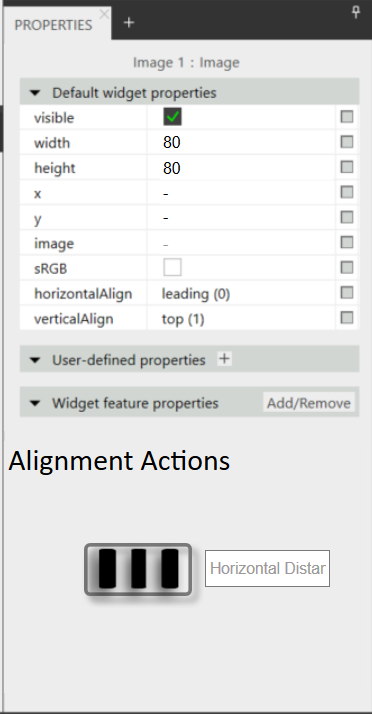
\includegraphics[width=0.3\linewidth]{figures/Prototyp_06.PNG}}%
\qquad
\subfloat[][]{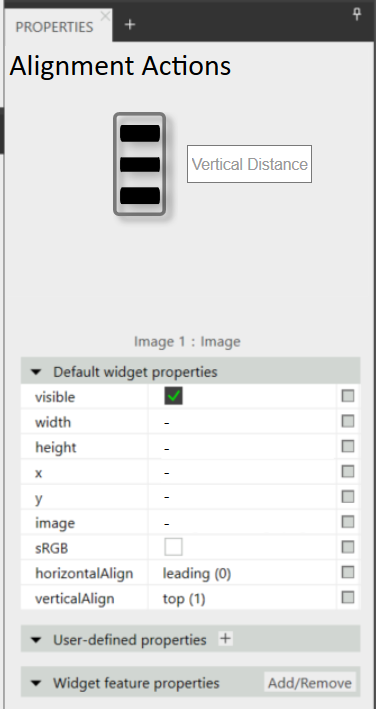
\includegraphics[width=0.3\linewidth]{figures/Prototyp_07.PNG}}%

\caption{Alignment Actions}%
\label{fig:Prototyp_06}
\end{figure}

Das Anlegen von Templates wird ebenfalls mit Screenshots simuliert die mit Hotspots versehen werden.
Zusätzlich besteht hier noch die Notwendigkeit einen Imagetab neben dem View anzulegen, da das Erstellen der Templates in einem anderen Bereich stattfindet.
In diesem Tab existiert ebenfalls ein Propertiespanel, die Funktion \glqq publish to template interface\grqq{} geschieht wie geplant über einen Klick auf den Kreis, der sich nach der Auswahl blau einfärbt.
Wird hier ein Wert angepasst wirkt sich das über eine globale Variable auch auf das Template Interface aus, eine Änderung im Template Interface darf jedoch nie ein Property des Templates anpassen.
Deshalb wurden hier zwei getrennte Sets von globalen Variablen angelegt, welche nur in eine Richtung synchronisieren.

\begin{center}
  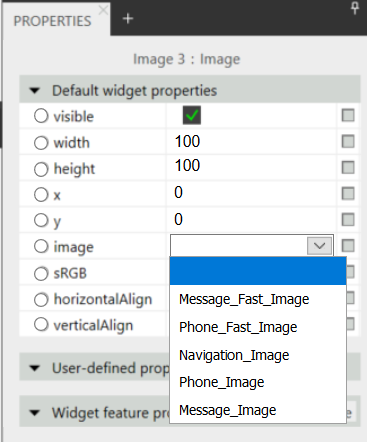
\includegraphics[scale=0.6]{figures/Prototyp_08.PNG}
  \captionof{figure}{Droplist für Images}
  \label{fig:Prototyp_08}
\end{center}

Die Zuweisung der Bilder im Template findet über ein Droplist statt, welches in \cref{fig:Prototyp_08} zu sehen ist.
Die Vorgehensweise, wie der sichtbare Inhalt eines Dynamic Panels mithilfe einer Droplist angepasst werden kann wurde bereits in Abschnitt 4.1.1 erklärt.
Anstatt der bunten Kreise befindet sich in diesem Fall jeweils eine Ausführung aller Bilder in den Dynamic Panels welche je nach Auswahl aus der Droplist sichtbar oder unsichtbar geschaltet werden.
Die Alternative Vorgehensweise \glqq Insert in Template\grqq{} funktioniert nach dem gleichen Prinzip.
Nur wird hier nicht aus der Droplist abgefragt, sondern welches Bild gleichzeitig mit dem Template ausgewählt ist.
Dieses wird dann nach einem Klick auf den Button entsprechend angezeigt.


\section {Implementierung Filter}
\subsection {Zielsetzung}
Optische und Funktionale Umsetzung des UX Design

\subsection {Projektaufbau}

Model-View-ViewModel (MVVM) 
\cite{.g}

CollectionViewSource
\cite{dotnetbot.}

\subsection {Vorgehensweise}

CollectionViewSource.Filter
\cite{dotnetbot.b}

\lstinputlisting[language=Python ,caption={Widget Properties Filter},captionpos=b]{listings/Filter.cs}

\lstinputlisting[language=Python ,caption={Filter Constructor},captionpos=b]{listings/Filter_Constructor.cs}

\lstinputlisting[language=Python ,caption={CollectionViewSource()},captionpos=b]{listings/ICollectionView.cs}

\lstinputlisting[language=XML,caption={Filterpanel in xaml},captionpos=b]{listings/Filter_Panel.xaml}


